\begin{figure}
\begin{minipage}{\textwidth}
\centering
\raisebox{-0.5\height}{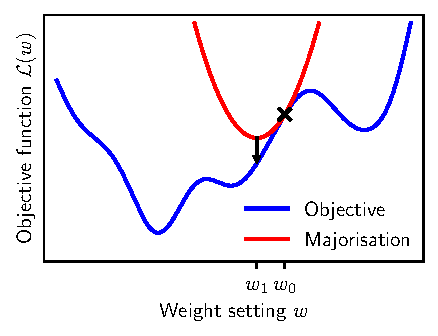
\includegraphics{figures/pdf/maj-min}} \hfill     \raisebox{-0.5\height}{
        \begin{tikzpicture}
        [thick, block/.style={draw, minimum size=1.1cm}]
        
        \node [block,fill=red!30]    (a)               {$\el$};
        \node [block,fill=green!30]  (b) [right =of a] {$\ell$};
        \node [block,fill=orange!30] (c) [right =of b] {$\vf$};
        \node [block,fill=blue!30]   (d) [right =of c] {$\vw$};
        
        \node [block,fill=red!10]    (u) [below =of a] {$\Delta \el$};
        \node [block,fill=green!10]  (v) [below =of b] {$\Delta \ell$};
        \node [block,fill=orange!10] (w) [below =of c] {$\Delta \vf$};
        \node [block,fill=blue!10]   (x) [above =of d] {$\Delta \vw$};
        
        \node (p) [left  =of x, align=right, xshift=0.8cm, yshift=-0.04cm] {perturbation applied\\by optimiser};
        \node (q) [below =of v, yshift=0.9cm, align=center] {$\underbrace{\hspace{14.5em}}$\\[0.5ex]perturbations induced by optimiser};
        \node [below =of d, yshift=0.9cm, align=center] {weights};
        \node [above =of c, yshift=-0.825cm, align=center] {model};
        \node [above =of b, yshift=-0.825cm, align=center] {loss};
        \node [above =of a, yshift=-0.89cm, align=center] {objective};
        
        \draw[-latex] (b) edge (a);
        \draw[-latex] (c) edge (b);
        \draw[-latex] (d) edge (c);
        
        \draw[-latex] (a) edge (u);
        \draw[-latex] (b) edge (v);
        \draw[-latex] (c) edge (w);
        \draw[-latex] (x) edge (d);
        \end{tikzpicture}}
\end{minipage}
\caption{\captiontitle{Majorise-minimise and the perturbation hierarchy.} The \captiontitle{left panel} depicts the majorise-minimise meta-algorithm \citep{mm}, which is an algorithmic pattern for reducing an objective (blue) by minimising a sequence of upper bounds (one shown in red). The upper bounds, known as a \textit{majorisation}, must lie tangent to the objective to guarantee an improvement in one step of the meta-algorithm. The \captiontitle{right panel} depicts the perturbation hierarchy of a generic machine learning model: the optimiser perturbs the weights and this induces perturbations to the model output, the loss on individual training examples and ultimately the overall objective. Majorising machine learning objective functions requires addressing the full perturbation hierarchy.}
\label{fig:maj-min}
\end{figure}